%%%%%%%%%%%%%%%%%%%%%%%%
% Einführung in §14a   %
%%%%%%%%%%%%%%%%%%%%%%%%

\section{Einführung in §14a}

\begin{frame}[allowframebreaks]{Hintergrund}
    \begin{block}{Was ist §14a EnWG (Energie-Wirtschaftsgesetz)?}
        Der \href{https://www.gesetze-im-internet.de/enwg_2005/__14a.html}{§14a} des Energiewirtschaftsgesetzes (EnWG2024\cite{EnWG2024}) regelt die steuerbare Nutzung bestimmter elektrischer Verbraucher im Stromnetz. Ziel ist es, durch eine netzdienliche Steuerung der Lasten Engpässe im Stromnetz zu vermeiden und eine effizientere Nutzung erneuerbarer Energien zu ermöglichen.
        Zudem werden variable Netzentgelte eingeführt.
    \end{block}

    \framebreak

    \begin{block}{Warum sind steuerbare Verbraucher wichtig?}
        \begin{itemize}
            \item Vermeidung von Netzüberlastungen
            \item Förderung der Energiewende
            \item Kosteneinsparungen beim Netzausbau
        \end{itemize}
    \end{block}

    \begin{block}{Warum sind variable Netzentgelte wichtig?}
        \begin{itemize}
            \item Vermeidung von hohen Netzlasten
            \item Verschiebung von Lasten in Niederlastzeiten
            \item Bessere Auslastung der Netzte
            \item ...dadurch weitere Kosteneinsparungen beim Netzausbau
        \end{itemize}
    \end{block}

    \framebreak

    \begin{block}{Auswirkungen auf Haushalte}
        \begin{itemize}
            \item Kosteneinsparung durch Verbrauch in günstigen Zeiten
            \item Teils Veränderung des Nutzerverhaltens nötig
            \item Direkter Einfluss auf eigene Netzkosten
            \item Erst mit SmartHome bzw. Energy Manager optimal nutzbar
        \end{itemize}
    \end{block}
    \begin{block}{Auswirkungen auf Netzbetreiber}
        \begin{itemize}
            \item Bedarf an intelligenten Messsystemen wächst
            \item Anforderung an IT-Infrastruktur
            \item Entlastung beim Ausbaubedarf an Netzknoten und Netzen
            \item Zwangsweise Umstellung auf digitalisierte Prozesse
        \end{itemize}
    \end{block}
\end{frame}

\begin{frame}{Rechtliche Grundlagen - Bundesnatzagentur}
    \begin{block}{Beschluss BK8-22/010-A}
        In §14a EnWG \cite{EnWG2024} hat der Gesetzgeber festgelegt, dass Verteilnetzbetreiber künftig variable Netzentgelte für steuerbare Verbrauchseinrichtungen anbieten müssen. 
        Die Pflicht zur genauen Festlegung wurde der Bundesnatzagentur übertragen, 
        welche bereits am 23.11.2023 den Beschluss BK8-22/010-A\cite{BNetzA-BK8-22-010-A} fasste.
    \end{block}
\end{frame}
   
\begin{frame}{Rechtliche Grundlagen - Beschluss BK8-22/010-A}

   Im Beschluss BK8-22/010-A\cite{BNetzA-BK8-22-010-A} der Bundesnetzagentur ist festgelegt, dass...
   \vspace{0.5cm}
   \begin{description}
      \item[Modul 1] eine jährliche Erstattung,
      \item[Modul 2] einen ermäßigten Tarif,
      \item[Modul 3] und ein variables Netzentgelt
   \end{description}
   \vspace{0.5cm}
   ...vom Netzbetreiber angeboten werden muss. 
\end{frame}
   
\begin{frame}{Rechtliche Grundlagen - Auswahl der Module}
    Hierbei kann/muss man wählen zwischen:
    \begin{description}
        \item[Modul 2] mit gesonderter Messung und reduziertem Arbeitspreis
        \item[Modul 1] mit pauschler Erstattung
        \item[Modul 1 \& 3] ...zusätzlich mit variablen Netzentgelten
    \end{description} 
    \vspace{0.5cm}
    \begin{block}{Festlegungen zur Ausgestaltung}    
        Hierbei wurden auch Festlegungen speziell zur Ausgestaltung des Moduls 3 getroffen bzgl. der Hoch- und 
        Niedertarifpreise und mindestens zweier Quartale (S.4 Abs.3c) pro Jahr mit variablen Netzentgelten.
    \end{block}
\end{frame}

\begin{frame}{Rechtliche Grundlagen - Vorgaben Modul 3}
   
   In der Anlage zum Beschluss (S.62) finden sich dann auch Details zur Tarifgestaltung.

   \begin{enumerate}
      \item Die Hochtarifstufe muss in mindestens 2 Stunden eines Tages abgerechnet werden 
         und darf die Standardtarifstufe um maximal 100\% übersteigen.
      \item Der Netzbetreiber hat eine Niedrigtarifstufe im Korridor zwischen 10 und 40\% der 
         Standardtarifstufe zu bilden.
      \item Ein hypothetischer Verbraucher mit einem dem Standardlastprofil für 
         Haushaltskunden (H0) identischen Verbrauchsprofil wäre bei einer existierenden 
         Wahlmöglichkeit indifferent zwischen dem Arbeitspreis für Entnahme ohne 
         Leisstungsmessung und dem Modul 3.
   \end{enumerate}
\end{frame}

\begin{frame}{Ergänzung - Haushaltslastprofil H0}
    \centering
    \begin{tikzpicture}
        \node[anchor=center] at (0, 0) {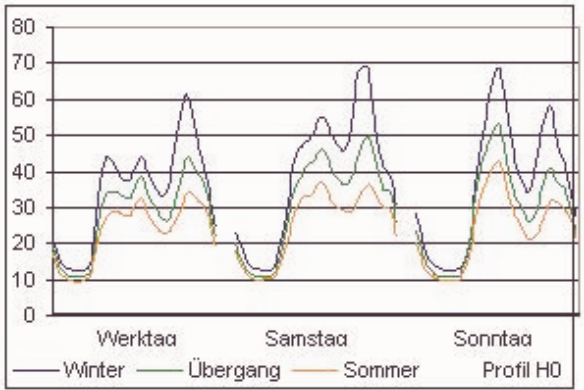
\includegraphics[height=0.70\paperheight]{images/Lastprofil_Haushalt_H0.png}};
        \node[rotate=90,anchor=center] at (5.5, 0) {Quelle: BDEW\cite{BDEW1999ReprLProf}};
    \end{tikzpicture}
 \end{frame}

 \begin{frame}{Stromerzeugung und Last - Winter}
    \centering
    \begin{tikzpicture}
        \node[anchor=center] at (0, 0) {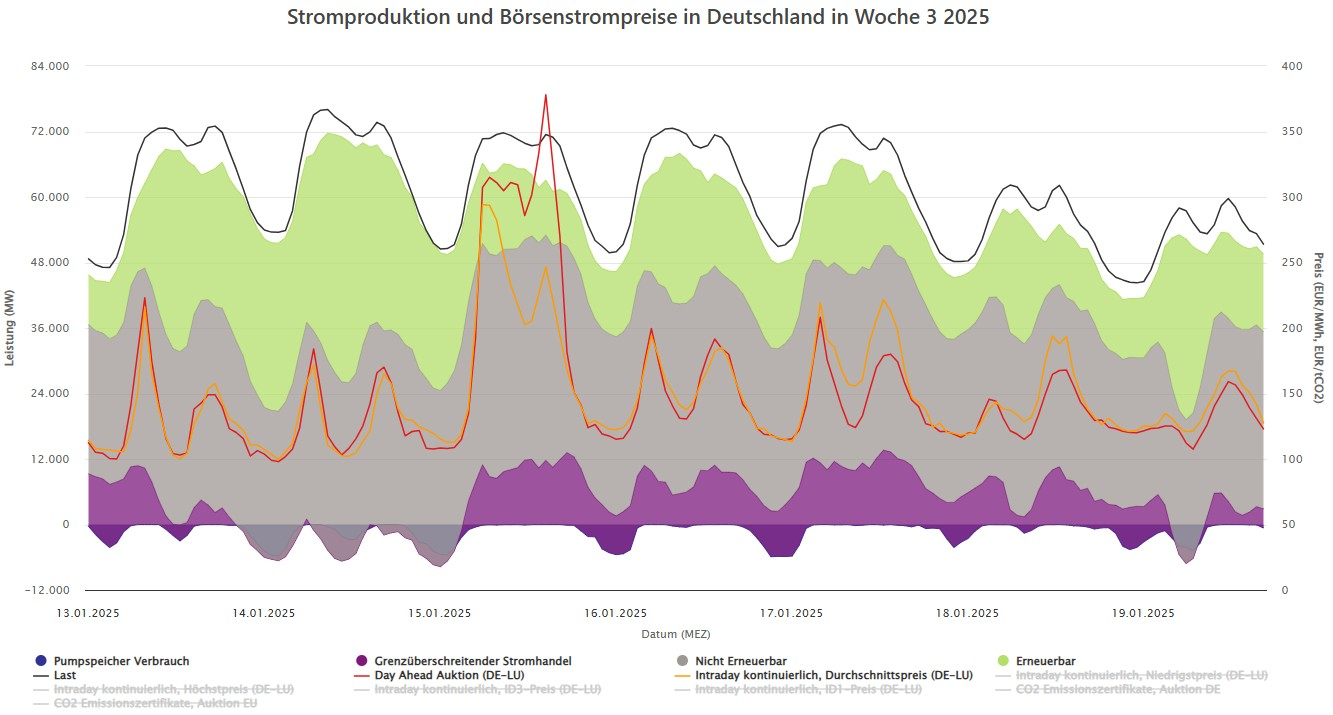
\includegraphics[width=0.9\paperwidth]{images/Stromproduktion_Winter.jpg}};
        \node[rotate=90,anchor=center] at (6, 0) {Quelle: Energy Charts};
    \end{tikzpicture}
\end{frame}

\begin{frame}{Stromerzeugung und Last - Frühling}
    \centering
    \begin{tikzpicture}
        \node[anchor=center] at (0, 0) {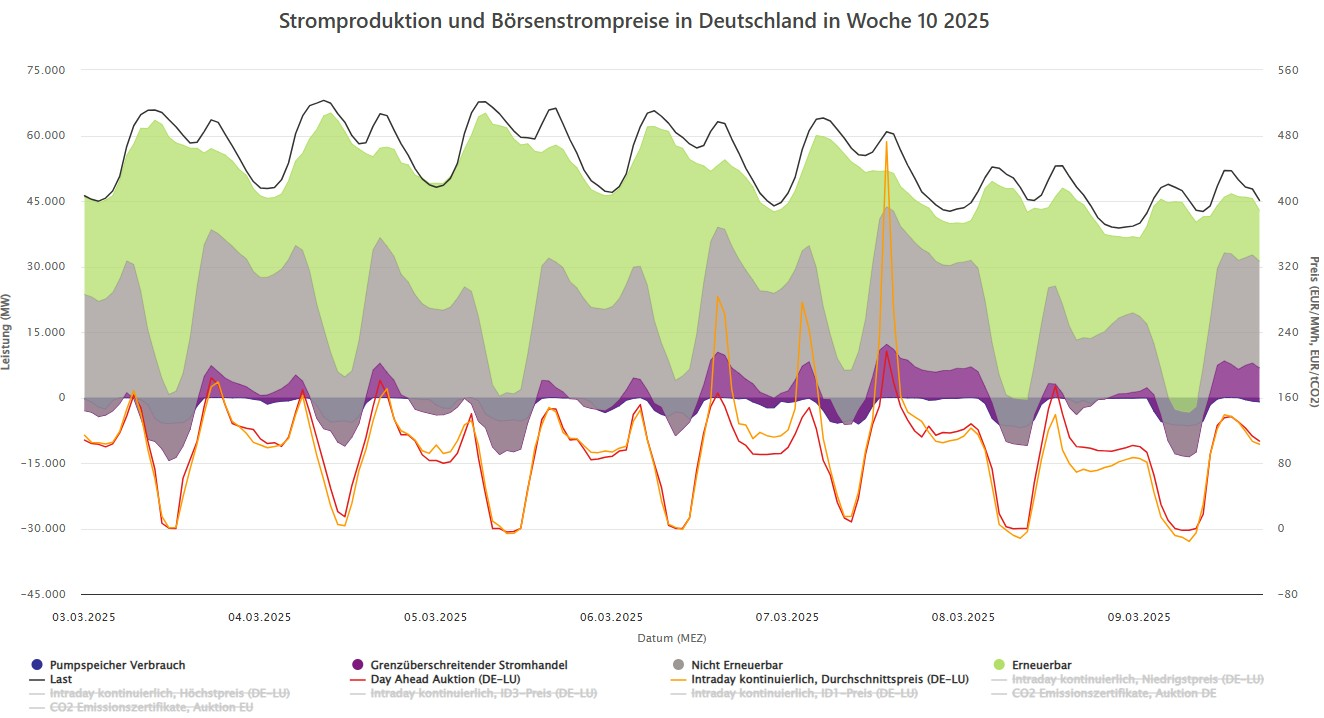
\includegraphics[width=0.9\paperwidth]{images/Stromproduktion_Fruehling.jpg}};
        \node[rotate=90,anchor=center] at (6, 0) {Quelle: Energy Charts};
    \end{tikzpicture}
\end{frame}

\begin{frame}{Stromerzeugung und Last - Sommer}
    \centering
    \begin{tikzpicture}
        \node[anchor=center] at (0, 0) {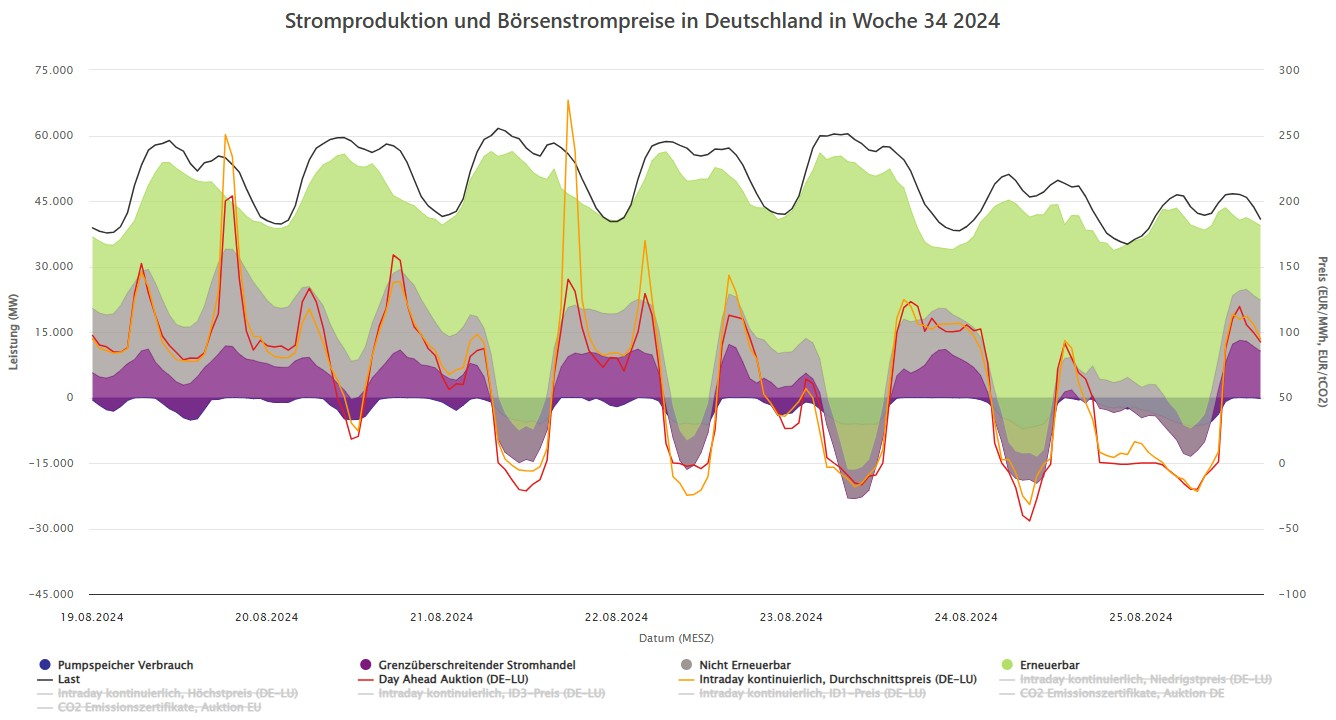
\includegraphics[width=0.9\paperwidth]{images/Stromproduktion_Sommer.jpg}};
        \node[rotate=90,anchor=center] at (6, 0) {Quelle: Energy Charts};
    \end{tikzpicture}
\end{frame}